\documentclass[grado3]{LEMA-Tikz-IM}

\usepackage{graphicx}  % Needed to include graphics

\begin{document}
\begin{tikzpicture}

% page canvas letter size
\path (0,0) rectangle (8.5in,11in);

\def\myMargin{1in}

\coordinate (botLeft) at (\myMargin,\myMargin);
\coordinate (botRight) at (8.5in-\myMargin,\myMargin);
\coordinate (topRight) at (8.5in-\myMargin,11in-\myMargin);
\coordinate (topLeft) at (\myMargin,11in-\myMargin);

% clip outside the margin
\clip (botLeft) rectangle (topRight);

% draw middle line
\coordinate (midLeft) at ($ (botLeft)!0.5!(topLeft) $);
\coordinate (midRight) at ($ (botRight)!0.5!(topRight) $);
\draw (midLeft)  -- (midRight);

% find center of top and bottom pieces
\coordinate (centerTop) at ($ (midLeft)!0.5!(topRight) $);
\coordinate (centerBot) at ($ (midLeft)!0.5!(botRight) $);

% add tables to top and bottom
\node (tableTop) at ([yshift=-1cm]centerTop) {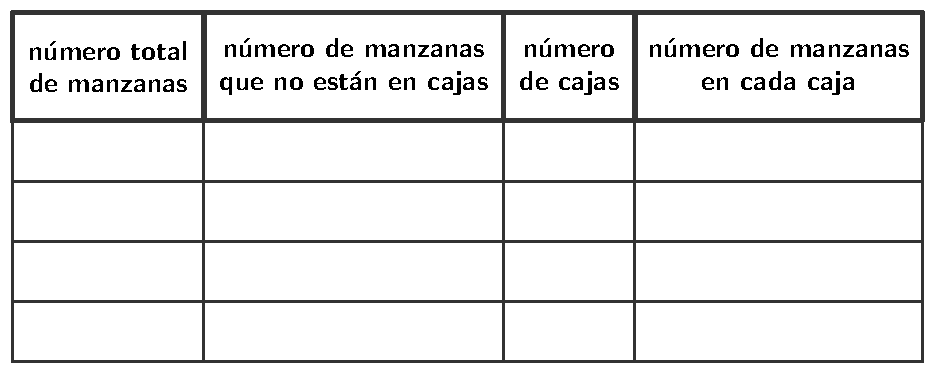
\includegraphics{3-4-21-act1-BLM-table.pdf}};
\node (tableBot) at ([yshift=-1cm]centerBot) {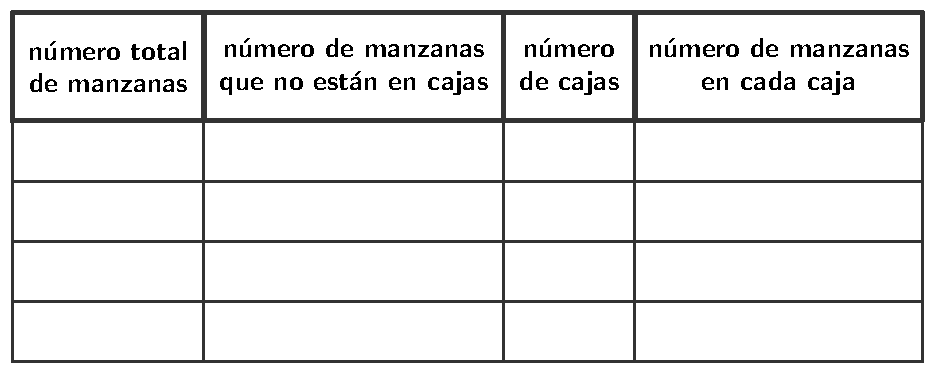
\includegraphics{3-4-21-act1-BLM-table.pdf}};

% Add png decoration to top and bottom
\node[above] at (tableTop.north) {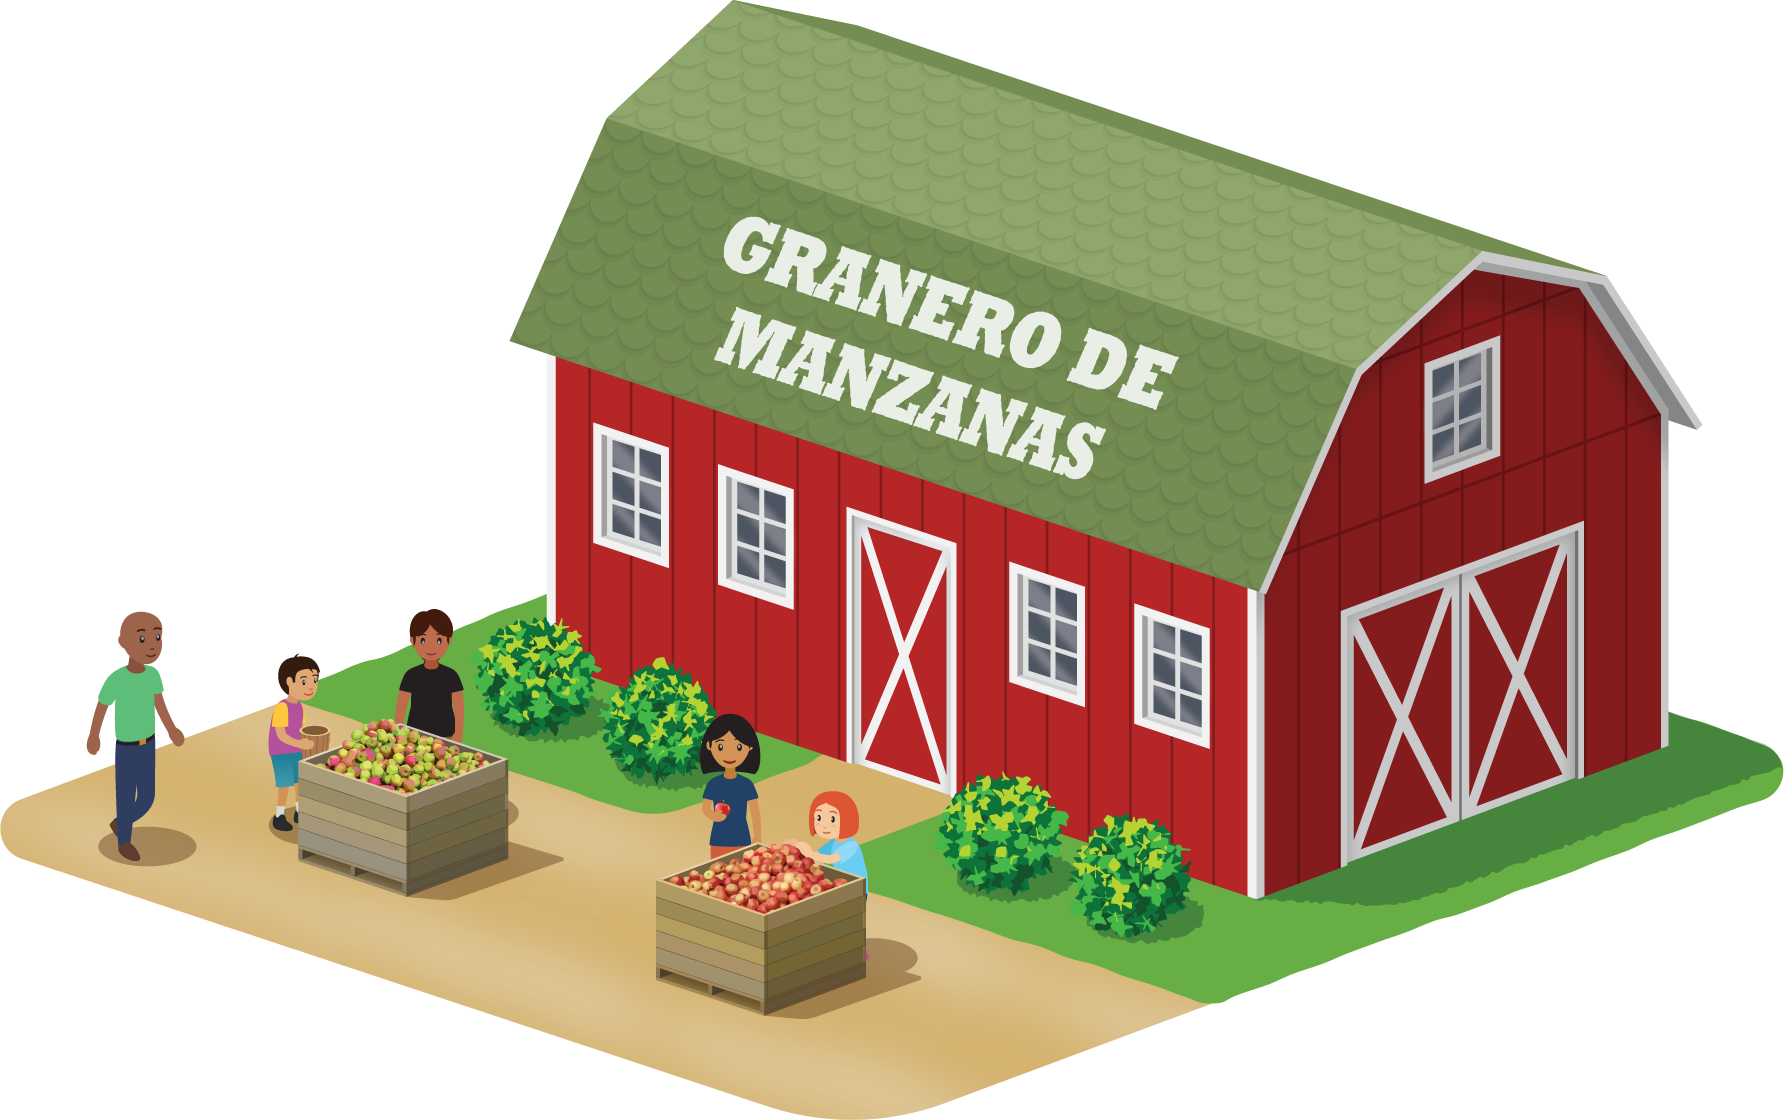
\includegraphics[width=2.5cm]{../../png-source/3.4.D21.S_Sp.png}};
\node[above] at (tableBot.north) {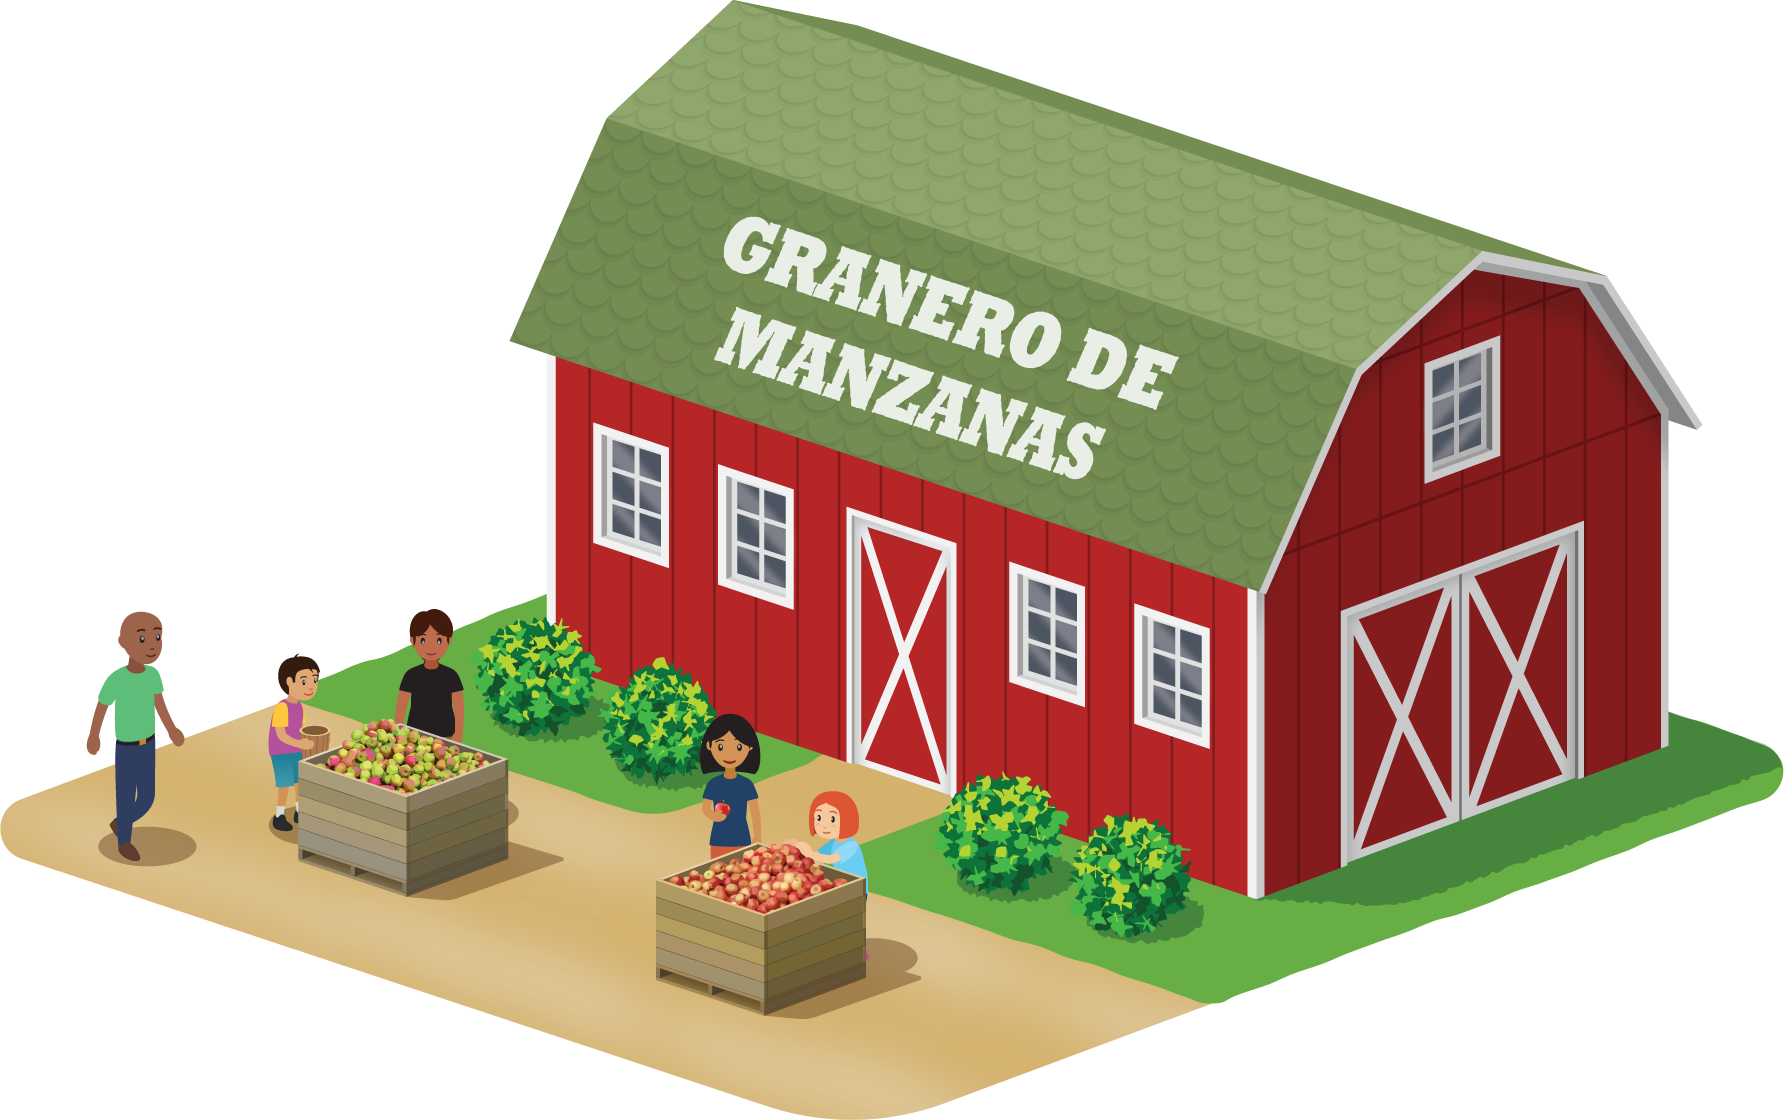
\includegraphics[width=2.5cm]{../../png-source/3.4.D21.S_Sp.png}};

% Add BLM heading to top and bottom
\node[below right] at (topLeft) {\bf Una aventura con manzanas};
\node[below right] at (midLeft) {\bf Una aventura con manzanas};


\end{tikzpicture}
\end{document}